%% Copernicus Publications Manuscript Preparation Template for LaTeX Submissions
%% ---------------------------------
%% This template should be used for copernicus.cls
%% The class file and some style files are bundled in the Copernicus Latex Package, which can be downloaded from the different journal webpages.
%% For further assistance please contact Copernicus Publications at: production@copernicus.org
%% https://publications.copernicus.org/for_authors/manuscript_preparation.html


%% Please use the following documentclass and journal abbreviations for preprints and final revised papers.

%% 2-column papers and preprints
\documentclass[npg, manuscript]{copernicus}


%% \usepackage commands included in the copernicus.cls:
%\usepackage[german, english]{babel}
%\usepackage{tabularx}
%\usepackage{cancel}
%\usepackage{multirow}
%\usepackage{supertabular}
%\usepackage{algorithmic}
%\usepackage{algorithm}
%\usepackage{amsthm}
%\usepackage{float}
%\usepackage{subfig}
%\usepackage{rotating}


\begin{document}

\title{Phytoplankton Retention Mechanisms in Estuaries: A Case Study of the Elbe Estuary}


% \Author[affil]{given_name}{surname}

\Author[1]{Laurin}{Steidle}
\Author[2]{Ross}{Vennell}
\Author[3]{Jana}{Hinners}

\affil[1]{Universität Hamburg, Olbersweg 24, 22767 Hamburg, Germany}
\affil[2]{Cawthron Institute, 98 Halifax Street East,
Nelson 7010, New Zealand}
\affil[3]{Helmholtz-Zentrum Hereon, Max-Planck-Straße 1, 21502 Geesthacht, Germany}

%% The [] brackets identify the author with the corresponding affiliation. 1, 2, 3, etc. should be inserted.

%% If an author is deceased, please mark the respective author name(s) with a dagger, e.g. "\Author[2,$\dag$]{Anton}{Smith}", and add a further "\affil[$\dag$]{deceased, 1 July 2019}".

%% If authors contributed equally, please mark the respective author names with an asterisk, e.g. "\Author[2,*]{Anton}{Smith}" and "\Author[3,*]{Bradley}{Miller}" and add a further affiliation: "\affil[*]{These authors contributed equally to this work.}".


\correspondence{Laurin Steidle (laurin.steidle@uni-hamburg.de)}

\runningtitle{TEXT}

\runningauthor{TEXT}





\received{}
\pubdiscuss{} %% only important for two-stage journals
\revised{}
\accepted{}
\published{}

%% These dates will be inserted by Copernicus Publications during the typesetting process.


\firstpage{1}

\maketitle



\begin{abstract}
    Phytoplankton is essential for the proliferation of estuarine ecosystems.
    However, little is known how estuarine plankton retain themselves in an environment that continuously washes them into unfavorable marine waters.
    We present a new individual-based Lagrangian model of the Elbe estuary examining several retention mechanisms - most importantly vertical migration and tidal stranding.
    We further examine their ability to outgrow losses and provide first estimates on outwashing losses.
    We found that shallow waters are crucial for the long term survival of the phytoplankton population.
\end{abstract}


% \copyrightstatement{TEXT} %% This section is optional and can be used for copyright transfers.


\introduction  %% \introduction[modified heading if necessary]
\texttt{Add a short paragraph as an outlook of the paper? I was told thats what the cool kids do, but I have a hard time getting it work.}


Estuaries are important both for the climate system and for anthropogenic use.
From a climate perspective they are highly productive relative to their surface area,
which results in large amounts of direct carbon cycling 
along with their important role as a source of nutrients and hatching grounds for marine ecosystem 
\citep{Cloern2014,Arevalo2023}
% (Phytoplankton primary production in the world’s estuarine-coastal ecosystems,Fish larvae dynamics in temperate estuaries: A review on processes, patterns and factors that determine recruitment). 
They are also strongly anthropogenically influenced through e.g. harbors, diking, dredging, fishing and pollution which can be seen as a stressor on the ecosystem, but also adds an anthropogenic dependency on the ecosystem. 
\citep{Jennerjahn2013, Brown2022, Wilson2002}
% (Pressures, stresses, shocks and trends in estuarine ecosystems: An introduction and synthesis,
% Anthropogenic-estuarine interactions cause disproportionate greenhouse gas production: A review of the evidence base,
% Productivity, Fisheries and Aquaculture in Temperate Estuaries)

Estuaries are also complex and strongly dynamic systems such that it is still difficult to predict ecosystem dynamics or the effects of anthropogenic changes.
This complexity arises in part from the bathymetrie and the resulting hydrodynamics at the model boundaries \citep{Michael2016, Fringer2019}. 
% (Sensitivity analysis of three-dimensional salinity simulations in North San Francisco Bay using the unstructured-grid SUNTANS model,
% The future of coastal and estuarine modeling: Findings from a workshop)

As for most ecosystems - their dynamics are strongly controlled by the primary producers \citep{Chen2023}
% (Advances in phytoplankton population ecology in the Pearl river estuary).
Phytoplankton, the 	predominant aquatic primary producer, is mostly drifting passively through the water.
Hence, its trajectory is strongly controlled by the currents and tides.
With the estuary having a net outwards flow, we would expect phytoplankton to be moving
 downstream over time and, ultimately, to be washed out into marine, high salinity waters.
Therefore, we are wondering how phytoplankton manage to survive as a population in such an environment.
If we assume that the population is not exclusively maintained by upstream plankton that is washed into the estuary,
 then there must be some sort of retention mechanism that enables a phytoplankton population to remain in the low-salinity area of the estuary.
While we suspect that such a mechanism is crucial for survival, it is currently not well understood 
due to the difficulty in either measuring or modeling such processes.



% \subsection{Current state of knowledge}


We categorize the already performed studies on the subject of phytoplankton retention in observational and modelling studies.

Observational studies have found three major mechanism for retention - sinking, diel migration, and stickiness.
Diel migration - moving up and down with the sun - has been found to be favorable for retention.
However, this only has been demonstrated for larger motile estuarine organisms i.e. zooplankton species \citep{Hall2015,Kimmerer2002, Crawford1991}
\citep{Anderson1985} was able to describe an estuarine embayment environnement in which dinoflagellates outcompeted other non-motile phytoplankton by  diel vertical migration.
They were also able to show that outwashing loses were lower than their growth rate - increasing their abundance.
However, this also implies that the growing part of the population is somehow retaining their position.
If the regrowing population is also continuously drifting downstream they will will not able to sustain their population in that area and ultimately die out due to unfavorable salinity conditions \citep{Admiraal1976, vonAlvensleben2016, Jiang2020}.
% (Vertical spatio-temporal patterns of phytoplankton due to migration behaviors in two shallow, microtidal estuaries: Influence on phytoplankton function and structure,
% Persistence of Tidally-oriented Vertical Migration by Zooplankton in a Temperate Estuary,
% Evidence for avoidance of flushing from an estuary by a planktonic, phototrophic ciliate, Flocculation kinetics and mechanisms of microalgae- and clay-containing suspensions in different microalgal growth phases).
Diatoms or benthic microalgea in particular have been observed to be strongly negatively buoyant, hence sinking to the ground and remaining there for a long time \citep{Passow1991}
% (Species-specific sedimentation and sinking velocities of diatoms).
Studies also found sticky compounds in phytoplankton aggregates that are suspected to let them stick to suspended particles making them sink to the ground or sticking to their surroundings aiding retention \citep{Kiørboe1993,VanderLee2000}.
% (Phytoplankton aggregate formation: observations of patterns and mechanisms of cell sticking and the significance of exopolymeric material,
% Parameters affecting mud floc size on a seasonal time scale: The impact of a phytoplankton bloom in the Dollard estuary)


Next we want to highlight several modelling studies that examined whether certain retention mechanism could work in theory.
% Two theoretical modelling studies examine the mechanisms of "loss compensation" and "reseeding".
% \texttt{I don't like the term theoretical modelling study. Maybe "conceptual", "abstract" or "simple"?}
% (Selective retention of two dinoflagellates in a well-mixed estuarine embayment: the importance of diel vertical migration and surface avoidance)
% \citep{Anderson1985} describes a set-up in which a population is able to maintain itself if the losses due to outwashing can be compensated by growth.
% In a environment where a lagoon like ecosystem was examined whether  they were able to quantify reproduction thresholds that are needed to maintain the population.
% However, this setup also implies that the growing part of the population is somehow retaining their position.
% If the regrowing population is also continuously drifting downstream they will also ultimately die out due to unfavorable salinity conditions \citep{Admiraal1976, vonAlvensleben2016, Jiang2020}.
% (Salinity Tolerance of Benthic Estuarine Diatoms as Tested with a Rapid Polarographic Measurement of Photosynthesis,
% Salinity tolerance of four freshwater microalgal species and the effects of salinity and nutrient limitation on biochemical profiles,
% Drivers of the spatial phytoplankton gradient in estuarine–coastal systems: generic implications of a case study in a Dutch tidal bay) 
% \citep{}
% studied the concept of "reseeding".
% Here a system is theorized in which a population is able to repopulate a previously 
% lost or uncolonized area upstream due to local upstream currents e.g. through tides or dispersion.
% While they showed that upstream reseeding is conceptually possible they did so in a specifically contrived system resembling groyne fields.
% Whether this is an actually realized phenomenon depends on the topology and hydrodynamic of the estuary.
% Nevertheless, it has been shown that both "outgrowing the losses" and "reseeding" are possible retention mechanism under certain conditions.
In \citep{Simons2006,Kimmerer2014} they use a particle tracking model also known as Lagragian model to study Zooplankton retention.
They were able to show that sinking and diel vertical migration slows the outwashing process and might be a beneficial retention tactic.
However, they did so by ignoring key processes like reproduction, mortality and any stranding or sedimentation processes in a low resolution structured grid model.

We are examining the Elbe estuary as a case study.
Like most alluvial estuaries it is relatively flat.
Similar to other European estuaries it experienced a strong anthropogenic pressure over the last centuries.
Most notably diking to restrain it to a narrow channel and dreading to improve access to the Hamburg harbor.
Unlike other major European harbors, the Hamburg harbor is located far inwards roughly 100 \unit{km} away from the coast.
This causes the river to experience a sudden jump in bathymetry from approx. 5 \unit{m} at border of the city to approx. 20 \unit{m} in the harbor (see fig. \ref{fig:bathymetry}). 
This bathymetric jump is suspected to be the cause of a collapse of the phytoplankton biomass causing an increase in oxygen depletion and high ammonium reminaralization after the bathymetric jump \citep{Schroeder1997,Holzwarth2018,Sanders2018}.
While major aspects of the along-channel biochemical dynamics have been studied little is known regarding their vertical and shore-to-shore dynamics.

\begin{figure}
    
\includegraphics[width=8.3cm]{figures/harbor.png}
    \caption{Bathymetry of the Elbe model around Hamburg. Note the bathymetric jumps from ~5 \unit{m} on the right, upstream side to a short 10 \unit{m} step in the upper harbor area to the ~20 \unit{m} in the lower harbor area all the way to the North Sea. Also note that there exists no channel that does not pass through the 10 \unit{km} of exclusively 20 \unit{m} deep channel.}
    \label{fig:bathymetry}
\end{figure}

To summarize - several concepts for potential retention mechanisms have been found
 and shown to work in certain conditions.
However, all approaches used major simplification which didn't allow them to study the full picture.
We developed a new and more realistic approach to study retention using a particle tracking model.
This model combines the features outlined above, namely: reproduction, mortality, vertical migration, stranding, sedimentation, and reseeding.
We examine if such a system can reproduce phytoplankton retention in the Elbe estuary with these mechanisms and if so under which conditions.


\section{Methods}
\subsection{Model description}

\subsubsection{Particle tracking}

In our study we take a particle tracking approach with a Lagrangian model called OceanTracker \citep{Vennell2021}.
Particle tracking offers several advantages for our question:
While particle tracking on unstructured grids has been relatively computationally expensive until recently \citep{Vennell2021}
it allows us to reuse already validated hydrodynamic models to model tracer like objects.
This approach is overall much faster than recalculating the advection-diffusion-equation in an Eularian model.

Additionally, because we are simulating individually particles we are able to observe their tracks.
This makes it much easier and intuitive to interpret the results and allows us to include individual based properties and processes.

\subsubsection{Hydrological model}
We use the hydrodynamics data of the most recent SCHISM model \citep{Pein2021}.
It is a three-dimensional unstructured  grid model representing the full Elbe estuary from the weir at Geesthacht to the North Sea including several side-channels and the harbor area (see fig. \ref{fig:model_domain}). 
% (Look for more details in pein paper that might be interesting)
The model provides a node-based mesh field containing a range of information.
Most important for our purpose is the water velocity but also salinity, water level and dispersion.
The year represented in that dataset is 2012 with 1h temporal- and dynamically varying spacial resolution with a median distance between nodes of approx. 60 \unit{m}.

\begin{figure}
    \includegraphics[width=12cm]{figures/dfg_foto_wettbewerbg_laurin_legendless_steidle_small.png}
    \caption{Map of the full model domain with Geesthacht being the upstream boarder on the right and the North-sea being the downstream edge on the top left. The gray outline indicates the edge of the model domain. Blue and green dots show an example snapshot of a phytoplankton distribution in the model. Blue being floating, green being stranded particles.}
    \label{fig:model_domain}
\end{figure}

\subsubsection{Particle based processes}

On top of the "blank" particle we add a set of biological features to achieve a more realistic planktonic behavior.
The most important one is their ability to reproduce by creating copies of themselves.
This is represented as a constant chance of duplicating a particle.
We also remove them under certain biologically unfavorable conditions. Specifically when they are stranded on the shore or starved for light or float in high salinity waters for too long.
More precisely, they are removed if either of the following criteria is met: 
When they reach high salinity waters above $10$PSU implemented as a mortality chance $1\%$ every minute.
When they are stranded outside the water and lie dry for more than $7$ consecutive days.
When they are starved for light which is represented as a budget of $14$ days 
where energy is lost in a fixed rate in low-light and gained in high light areas.
\texttt{I got these numbers from you - do you have a reference or reasoning for them?}

A set of vertical movement features is added to represent migration behavior. 
This is implemented in two modes. 
One is a constant vertical velocity i.e. sinking and rising
The second is diel vertical migration where they move up and down depending on the phase of the sun.
A large area of the estuary is very shallow with average water depths of below one meter. 
We include a simple sedimentation and resuspension model to represent stranding by the tide and also sedimentation model for the water column where resuspension is depending on a critical sheer velocity (see appendix).

Particles are stranded and temporarily stuck in place when they cross a model boundary or when their current location falls dry. 
Particle are resuspended from the bottom based on a critical sheer velocity model.
If they are stranded they resuspend as soon as there location is flooded again.

The model also implements dynamic dispersion that is crucial to represent tidal-pumping processes and to allow for more realistic trajectories.

\subsection{Experimental configurations}

The first experiment of this study examines retention success under different scenarios.
The general idea is to release a population of plankton at beginning of the estuary represented by the weir in Geesthacht.
We then examine how the population distributes itself over the estuary and whether it is able to maintain its population size.
% With this approach we study the effect of two retention mechanism in a sensitivity analysis. These being reproduction and migration.
The initial particle batch that is representing our phytoplankton population is released at the beginning of the year.
We evaluate their retention success by counting the amount of plankton in different regions in the estuary over time.
If the population is growing at the end of the year we consider them "successfully retained".
Population changes are measured at the end of the year relative to the population size after an initial spin-up time of three months when most of the initial batch has been washed out and the population is typically at its minimum.

For each particle we log their distance traveled, age, water depth, and status - whether they are drifting, stranded on the shore or bottom.
This allows us for example to compare successful (died older than three months) and unsuccessful (died younger than three months) plankton individuals.
The logged observables are measured every 12 hours starting at midnight.

\medskip

We use this set-up in a range of scenarios.
We call the first and simplest scenario "dust". 
Here we do not allow for any reproduction and give all particles a neutral buoyancy.
Hence, they are drifting like dust similar to a passive tracer.
This is our reference for any retention strategy. 
For a retention strategy to be considered beneficial it must perform better than these passive tracers.

In the second scenario referred to as "migration" reproduction is re-enabled.
In this scenario we study the effect of different growth rates and buoyancies i.e. vertical velocities on the phytoplankton population in a sensitivity analysis.

The third scenario has been added for illustration purposes.
Here, we use the same set-up as in the second scenario with the only exception of disabling reproduction for particles stranded on the shores of the estuaries.

% \subsubsection{upstream migration}

% In the second and minor experiment we test the hypothesis of "reseeding" - whether organisms can recolonize previously lost upstream habitats.
% \texttt{This is currently not included anymore. Seemed to uninteresting and far off track. What do you think?}


\subsection{Results}

\subsection{Retentions success in different scenarios}


\begin{figure}
    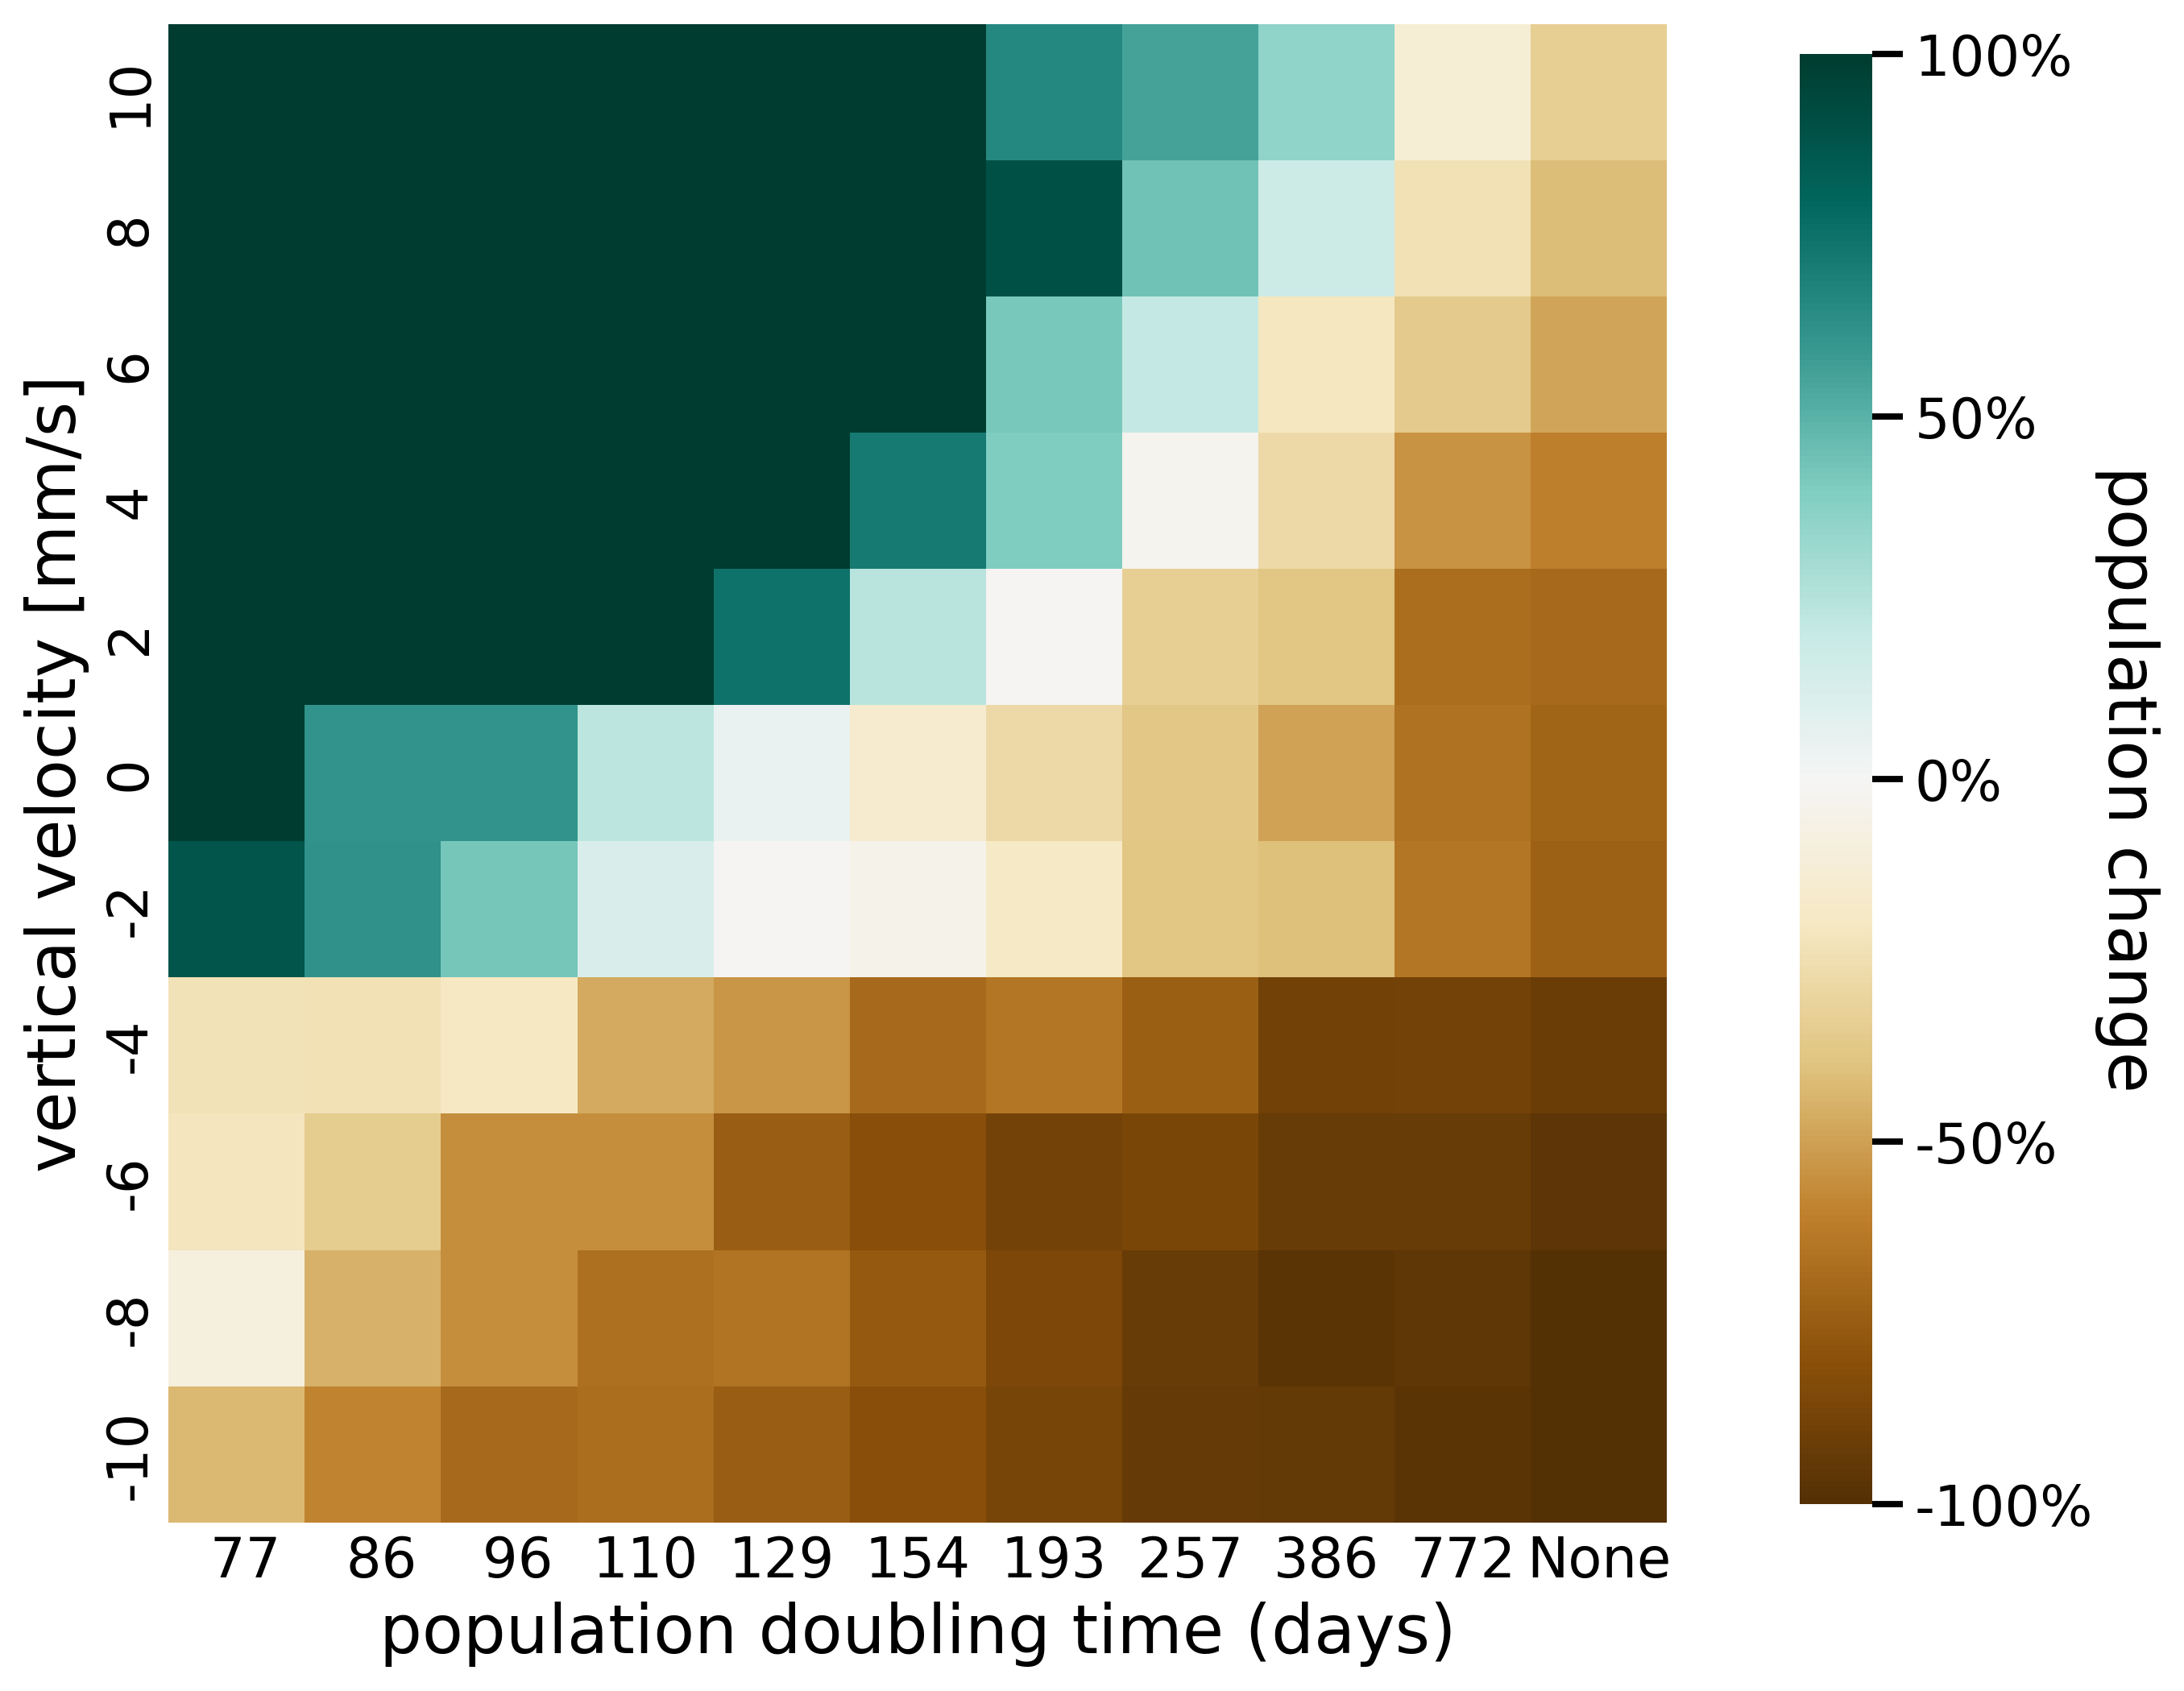
\includegraphics[width=8.3cm]{figures/retention_success_sa_mono.png}
    \caption[]{Relative population changes for the monotonic migration scenarios. Positive vertical velocities indicate an upwards drift. Positive population changes indicate a retention success (shown in green) while negative population changes predict a long term loss of the population (shown in brown).}
    \label{fig:monotonic_retention_success}
\end{figure}
\begin{figure}
    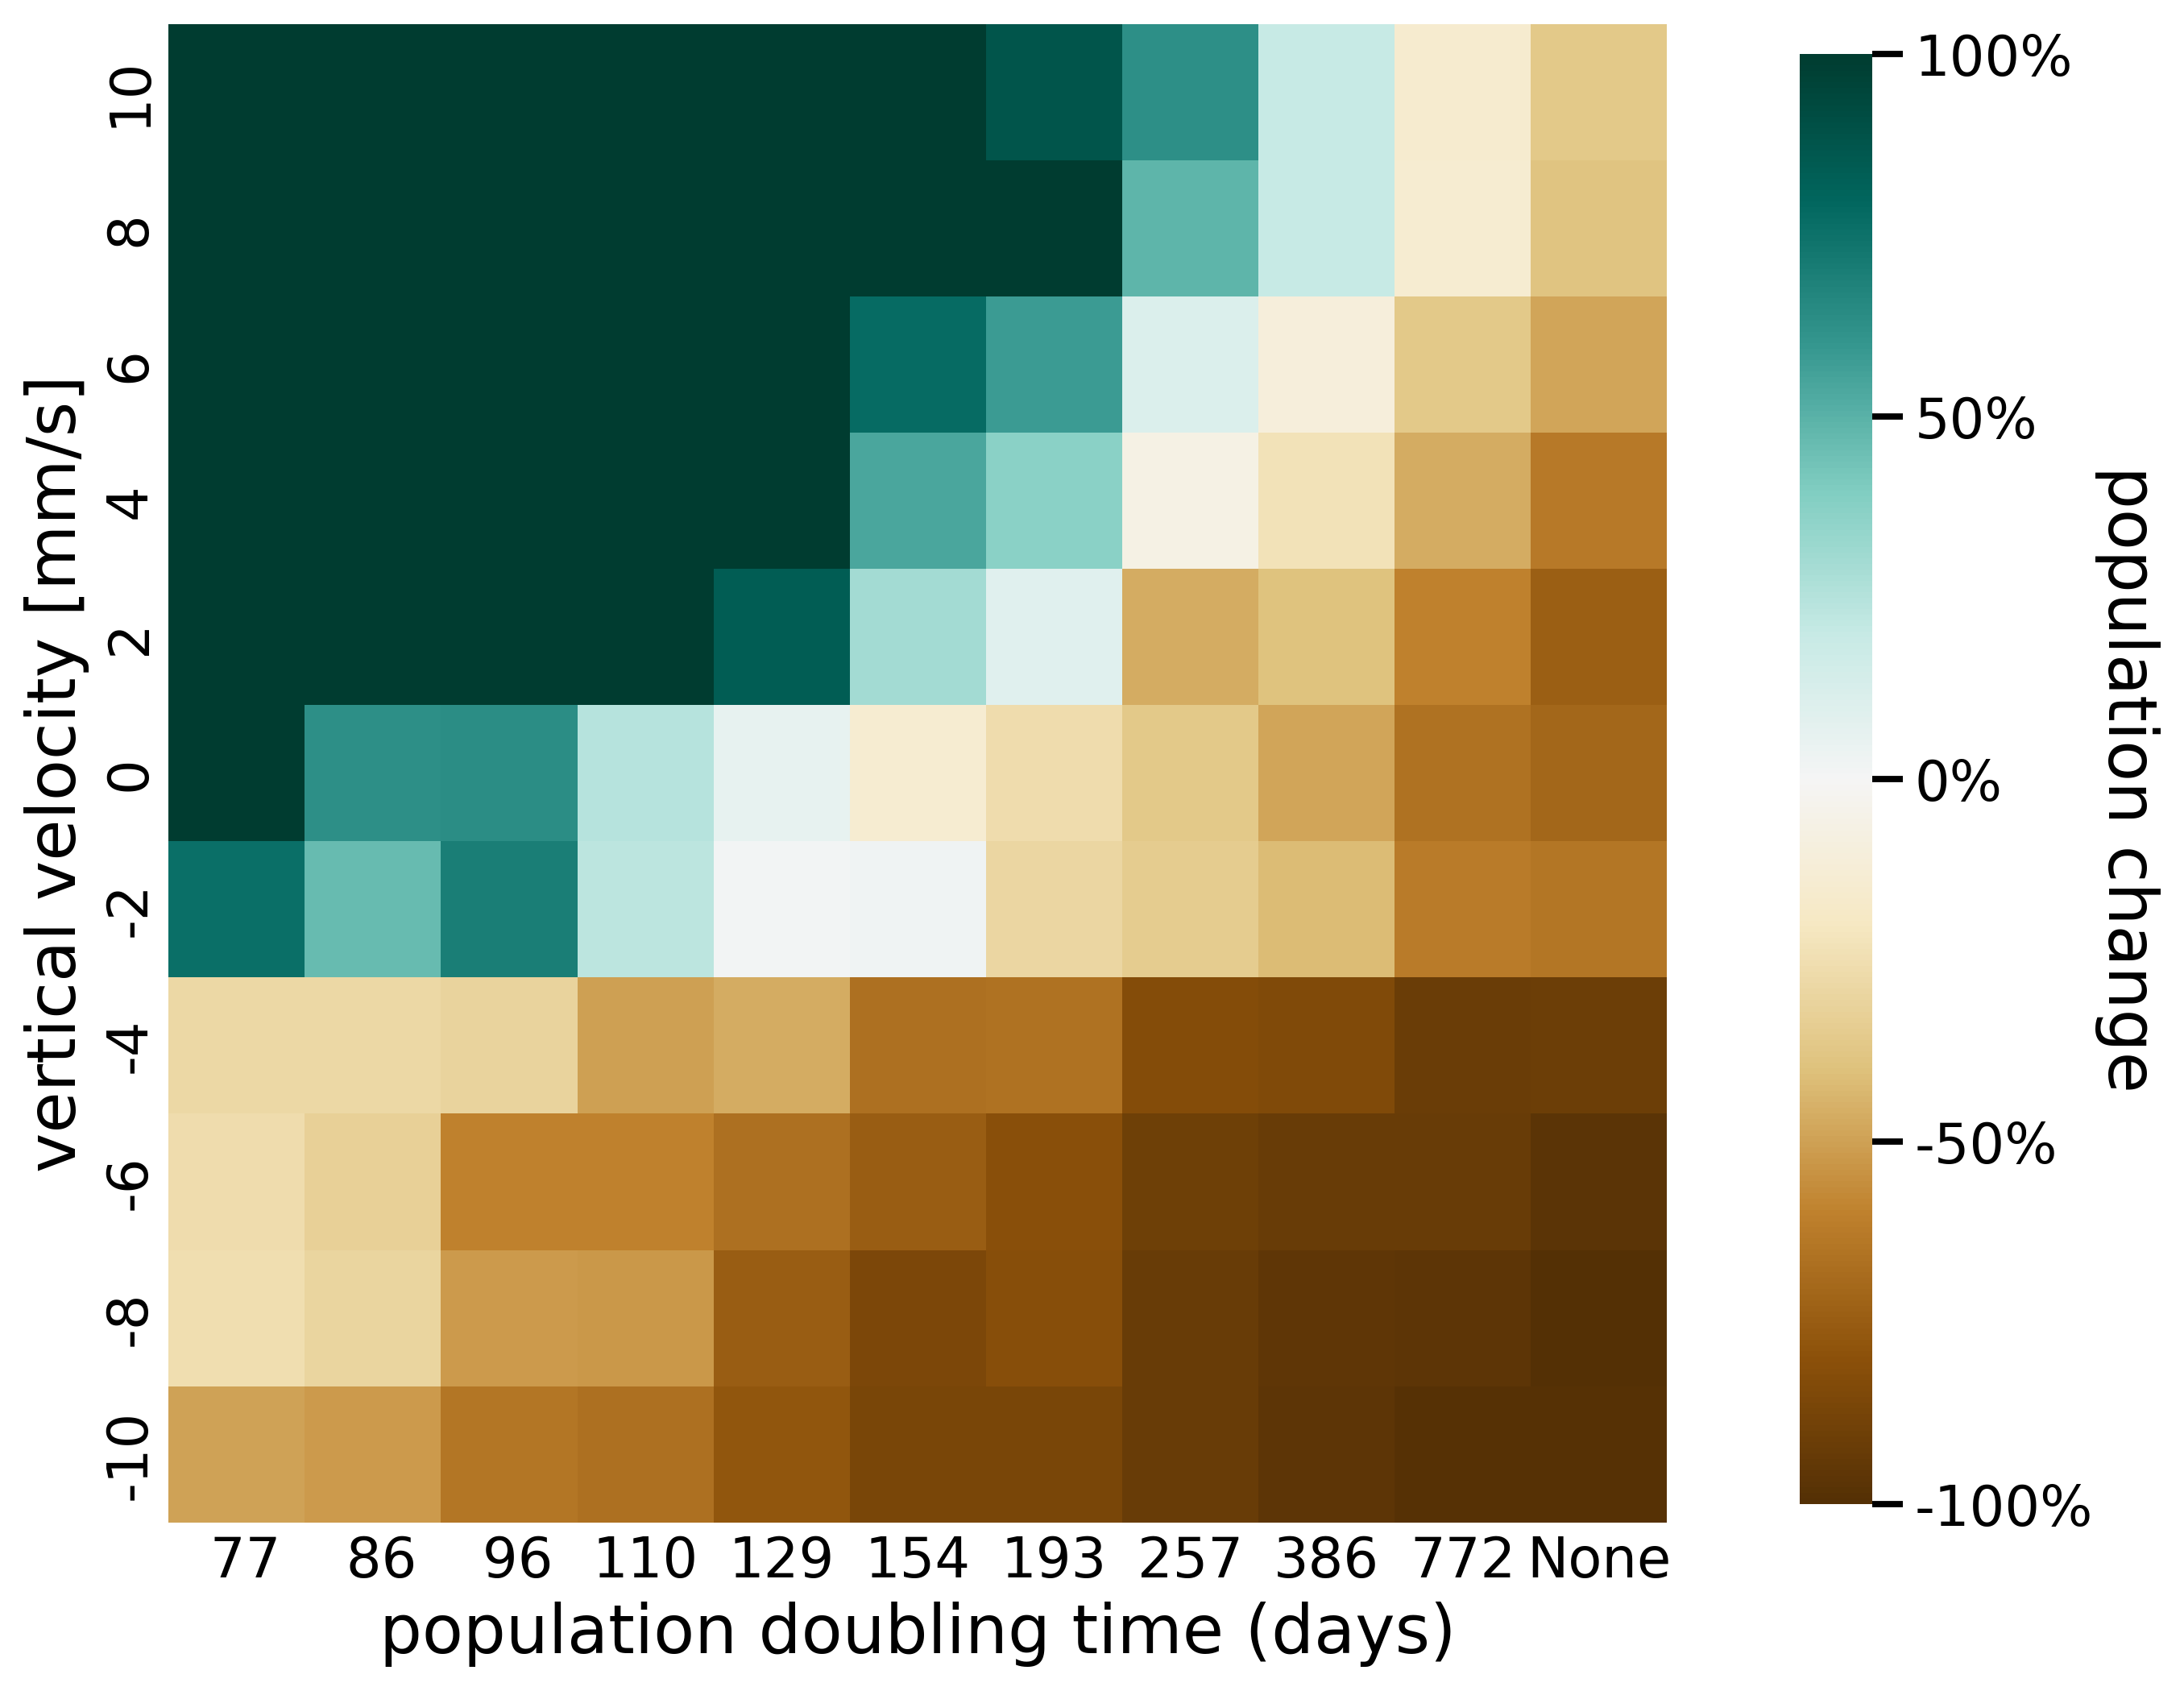
\includegraphics[width=8.3cm]{figures/retention_success_sa_diel.png}
    \caption[]{Relative population changes for the diel migration scenarios. Positive vertical velocities indicate an upwards drift. Positive population changes indicate a retention success (shown in green) while negative population changes predict a long term loss of the population (shown in brown).}
    \label{fig:diel_retention_success}
\end{figure}

The results of the retention experiments are visualized as heatmaps in fig. \ref{fig:monotonic_retention_success} and \ref{fig:diel_retention_success}.
Fig. \ref{fig:monotonic_retention_success} shows the results for the monotonic vertical migration scenarios e.g. constant sinking or rising.
Fig. \ref{fig:diel_retention_success} shows the results for the diel vertical migration scenarios. For the monotonic case a positive vertical velocity indicates an upwards motion. For the diel migration case a positive vertical velocity means that the particles are moving upwards during the day and downwards during the night.
Each pixel in the heatmap represents a scenario with a specific combination of vertical velocity and growth rate.
The coloring indicates the relative population change after one year. A positive (green) value is considered a successful retention while a negative (brown) value indicates that the population is dying out.

The first thing that we wish to highlight is that the population successfully retains itself in certain scenarios. For the case of the monotonic migration we see a trend that the populations with higher positive velocities and higher growth rates are more successful in retaining themselves.
For the case of the diel migration we see a trend to higher vertical velocities both upwards and downwards.

Another thing that we would like to point out is that populations with no reproduction are all unsuccessful in retaining themselves.

We would also like to note that a white pixels or the boundary between green and brown are scenarios with a net-zero growth rate. Because in this case the losses must be equal to the growth we can use the growth rate as an estimate for the total relative losses due to outwashing, dry-out when stranded, and light starvation.

\medskip

In the scenario where we disabled reproduction for stranded particles we found that the population was unable to retain itself in all tested parameterizations.


\subsection{Where do they survive?}

\begin{figure}
    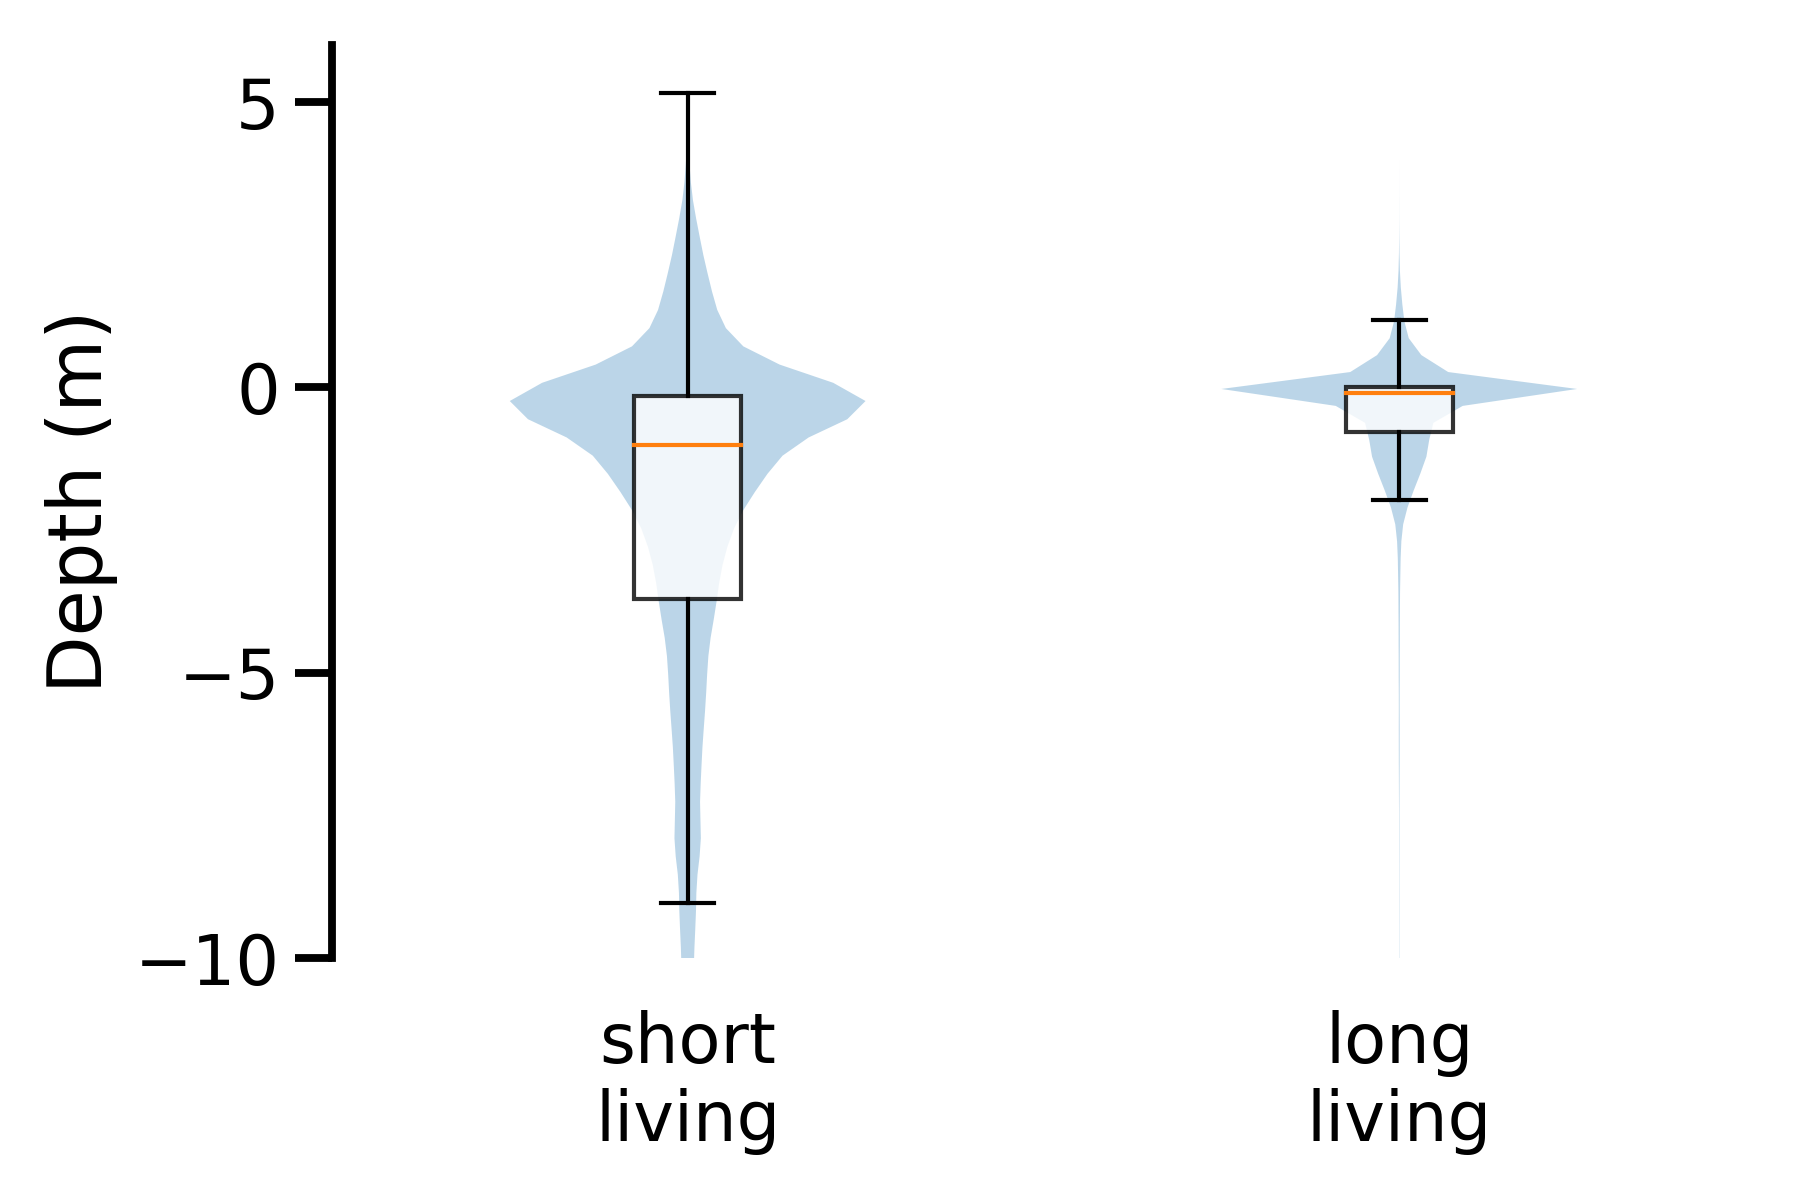
\includegraphics[width=8.3cm]{figures/retention_boxplot.png}
    \caption[]{Box and violin plot showing the vertical distribution of particles.  Short-living are those younger than 3 months and long-living all those older than that. Depth is measure relative to the current water surface with positive numbers being above the water surface i.e. stranded on shore.}
    \label{fig:migration-long-vs-short}
\end{figure}

We are now taking a closer look at the subset of phytoplankton that was able to retain themselves.
In fig. \ref{fig:migration-long-vs-short} we see a box plot comparing the average water depth at particle location for the long living and short living subset. The long living being older than three months.
Depth is measured relative to the water surface. Hence, a value above zero indicate that the particle is stranded on the shore.
We can clearly see that the long living subset predominantly lives close to the shores in shallower water.

\begin{figure}
    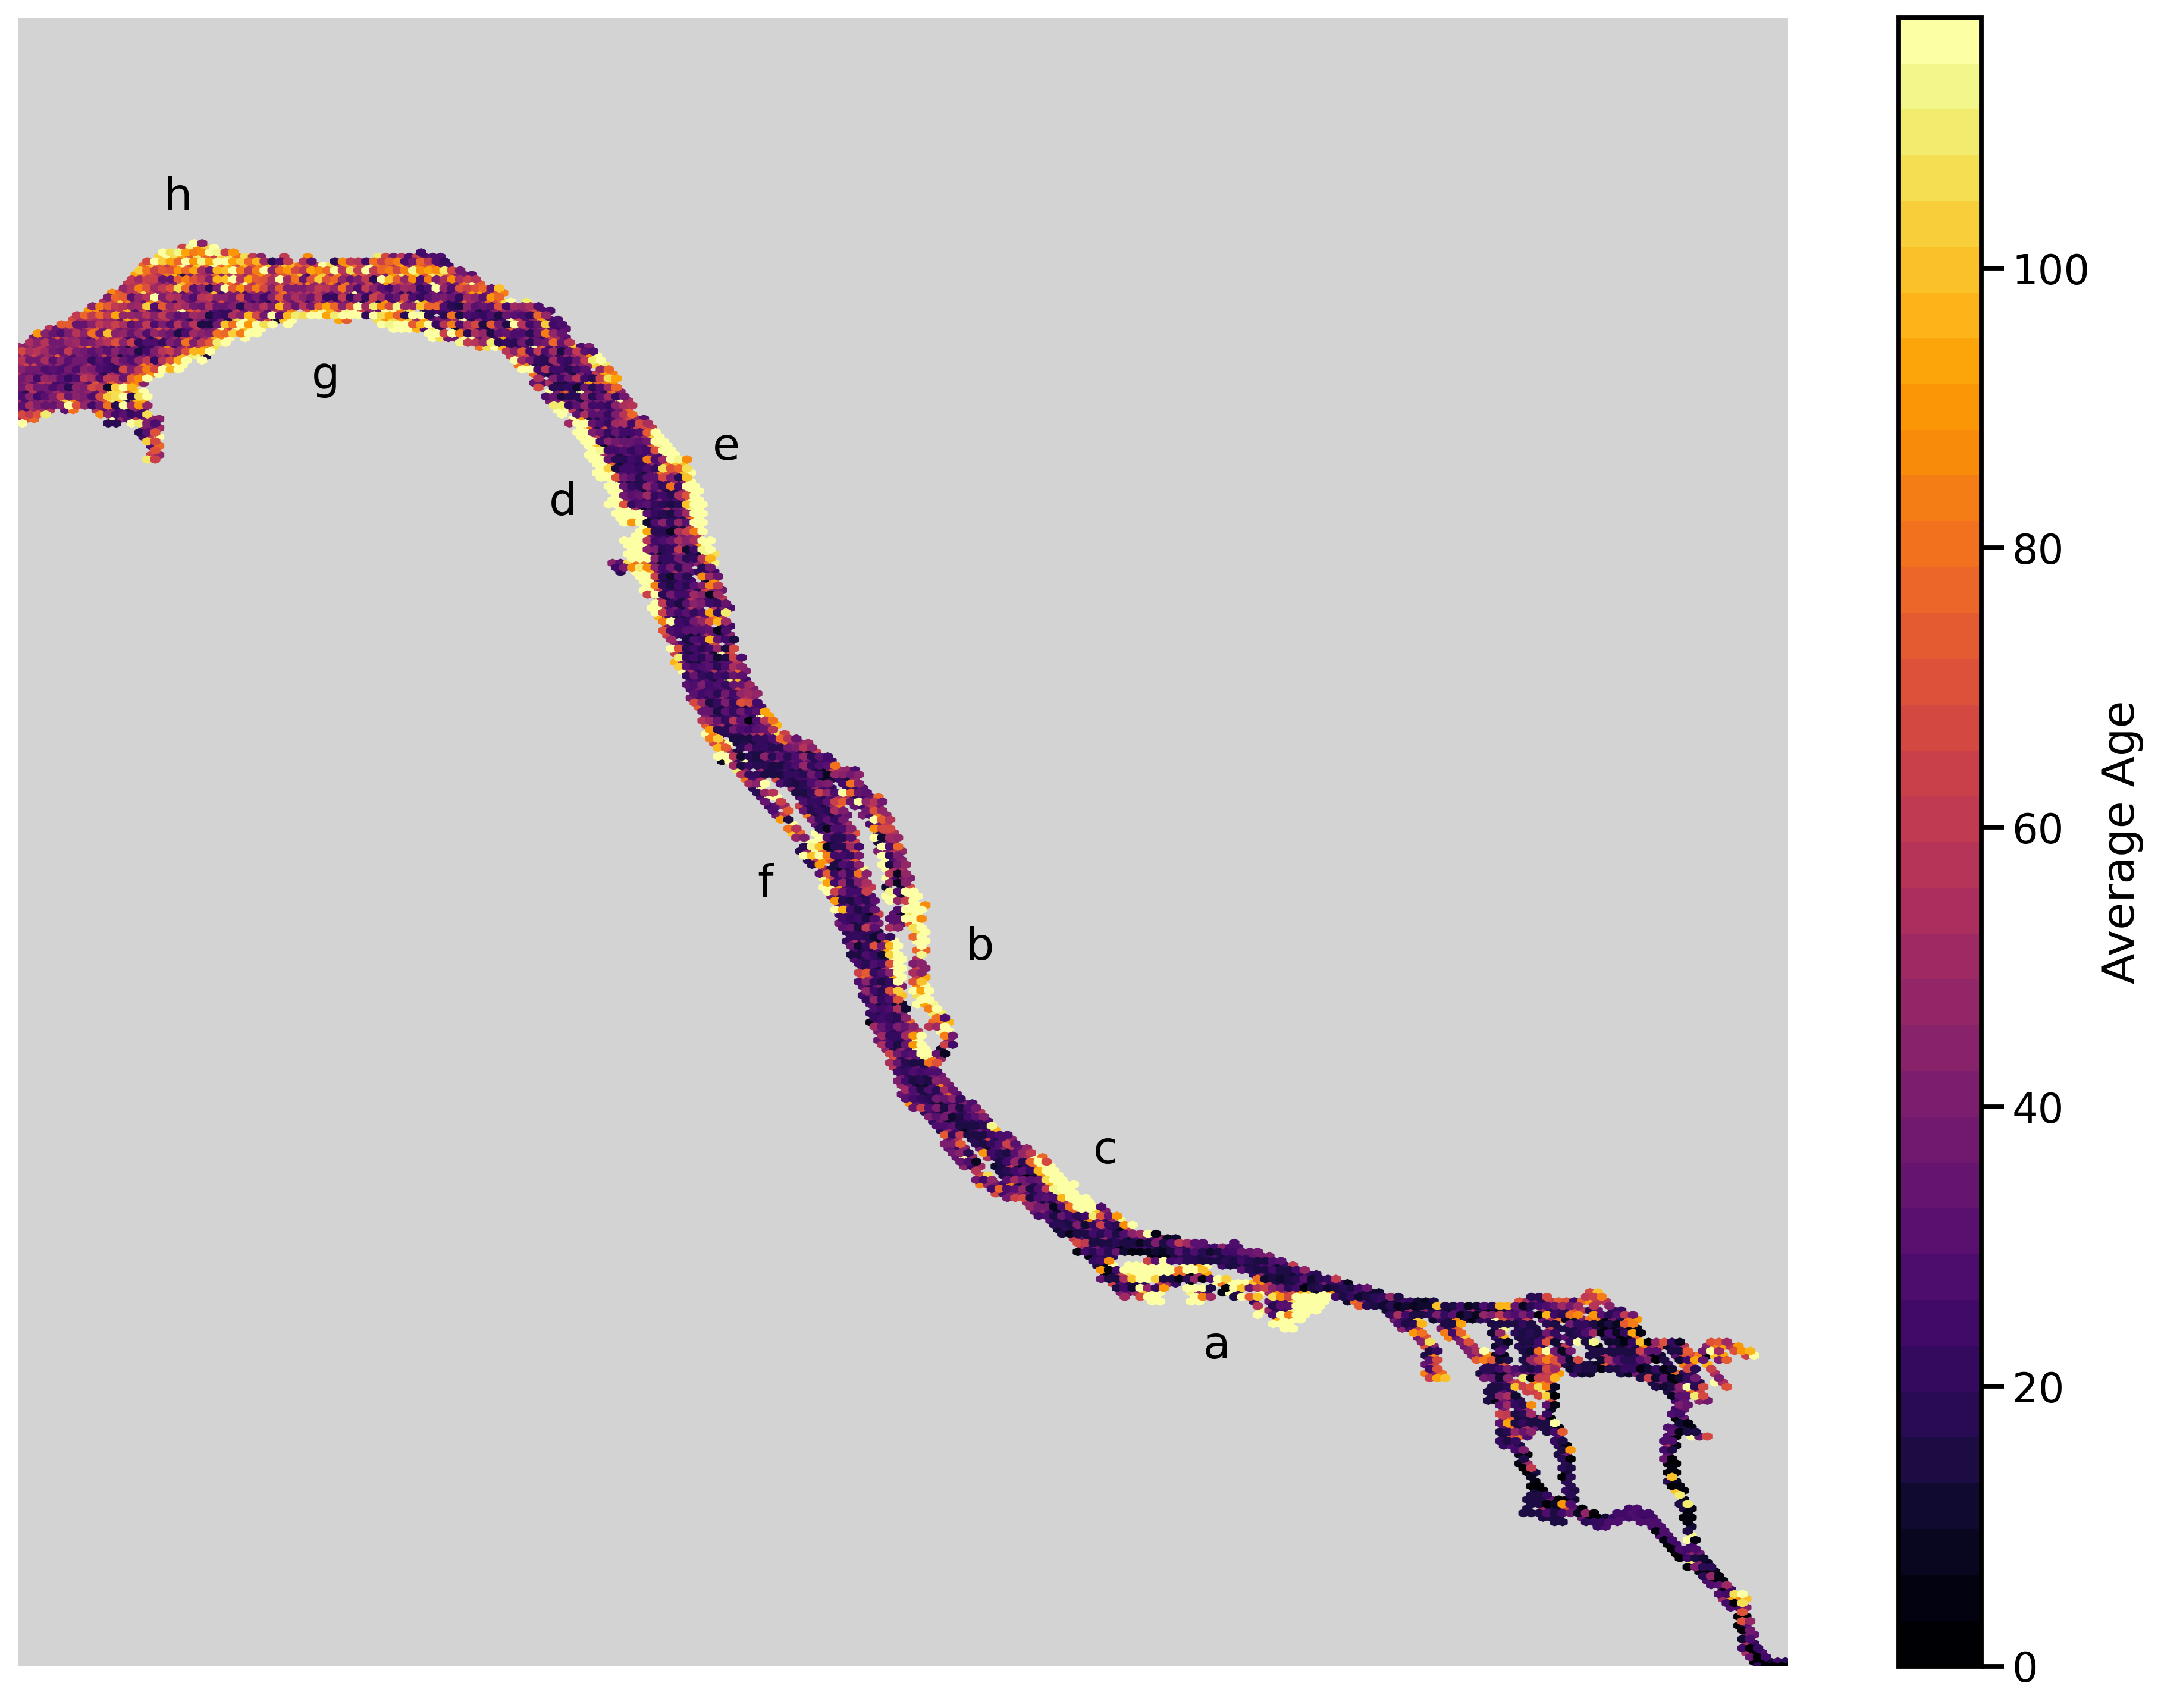
\includegraphics[width=8.3cm]{figures/age_hexbin.png}
    \caption[]{Hexbin heatmap of the Elbe with Hamburg in the bottom right showing average particle age per bin.  Yellowish colors indicate an average age of over three months.}
    \label{fig:migration-long-vs-short-heatmap}
\end{figure}

This is further supported by fig. \ref{fig:migration-long-vs-short-heatmap}.
Here we see a hex-bin-plot of the estuary. The coloring shows the average age of the particles in the bin.
Bins with an average age of over three months are shown in a yellowish color.
These yellow areas can exclusively be found along the shores in shallow areas.
The major areas being Mühlenberger Loch (a) and the Haseldorfer Binnenelbe (b). We can also find minor areas at Wedeler Marsch (c), at the mouth of Wischhafener Süderelbe (d), Ruthenstrom, and Stör (e), and at Nordkedding (g) and Neufelder Marsch (h).




\subsubsection{Discussion}

\subsection{Interpretation and contextualization of Results}

The range of growth rates that we found to be necessary for survival are small compared to those typically realized in nature where plankton populations can double their size in a day in ideal conditions.
Our model is simplistic in the sense that we do not include any nutrient limitation which are assumed to drastically decrease the growth rates compared to ideal conditions. 
Nevertheless, the growth rates that we found to be necessary are still much smaller compared to those typically realized in nature \citep{Koch2004}.

The importance of shallow near-shore areas for retention has been suggested several times by our findings. 
We assume that this is for the following reasons.
Plankton that lives in this area falls dry on the shore on a regular basis due to the tides. Hence, they are not moving downstream for a large portion of the day.
We further see that positively buoyant plankton is more successful in retaining themselves. 
This is likely due to the fact that they are more likely to be washed up high up at shore where the water reaches them less frequently.
This effect is emphasized in flatter regions.
In flatter regions the distance between the wash margin and constantly flooded areas is larger. 
We assume that this effect would be further emphasized if we were to represent Stokes drift in our model even though wind forcing on the surface water is included.

Initially we expected that negatively buoyant plankton would be more successful in retaining themselves.
Sinking particles have a reduced downstream velocity as they tend to get stuck on the ground more often.
Additionally, the bottom water layer in the Elbe typically has higher upstream velocity compared to the upper water column.
However, they still seem to be less successful than positively buoyant particles.
Examining our model we think  that this is because they tend to quickly aggregate in deep waters with little to no light where they are unable to sustain themselves and ultimately die out.
This is hinting at the negative impact of dredging on sinking plankton as it both increases depth and turbidity increasing the volume of dark water relative to the amount of illuminated waters.

Interestingly, diel migration success does not seem to depend on whether they are moving up during day or night.
We assume that this is to a large part due to them only surviving in shallow near-shore waters anyway where light limitation does not play a significant role.
We think the reason for higher success with higher vertical velocities is similar to the constant vertical velocity case.
When the upwards diel migration aligns with a high tide the particles are more likely to be stranded far out onto the shore decreasing their risk to be washed out quickly.
The higher the upwards velocities the higher the chance to be in the utmost part of the water body during high tide.
However, we also want to note that our light limitation model is very simplistic to keep the model complexity low.
For plankton not to be light limited they only need to be above a depth of one meter regardless of current illumination conditions and local turbidity.
Therefore, a more realistic light limitation model might introduce a positive bias towards those particles that move upwards during the day.

\subsection{Limitations of the model}

One major limitation of our model is the lack of nutrient limitation or the lack of a realistic ecosystem model in general.
This could have been done by coupling our Lagrangian model online to an Eularian model that would have advected changes in concentrations fields by biotic activity throughout the model domain.
However, this would have drastically increased both developing and computational time to a point where it would have been infeasible in our time frame and due to the lack of appropriate validation data.
The key draw back of this is that growth rates could only be modeled as a constant rate assuming an "ad libitum" environment at all times.
This introduces systematic errors in the population growth. In reality, areas which are beneficial for retention might run out of nutrients quickly and could not sustain the growth conditions necessary to sustain the local population.

Another major limitation is the lack of any sub-grid-resolution structure on the shores - especially vegetation.
In our representation we assume perfectly flat surfaces with a median distance between nodes of approximately 60 \unit{m}.
This "polished" model representation is assumed to cause a strong negative bias towards retention success as some plankton could easily stick to the vegetation or other cavities caused by the sub-grid-resolution structure and reseed the area.

While our model does have a sedimentation and resuspension mechanic based on critical sheer velocities we still assume a static bathymetrie with sediments not able to move or bury particles. 
This masks potential losses due to particles being buried but also decreases resuspension times.

\subsection{Outlook}

Our results clearly suggested the importance of shallow near-shore areas for the survival of phytoplankton in the Elbe estuary.
After our initial experiments suggested this, we considered improving our model to resolve additional ecosystem interactions especially nutrient limitation.
This would allow us to predict the population dynamics more realistically to the point where we would be able to quantize the importance of shallow areas more accurately.
However, the main limitation to do so was the lack of validation data for these regions. 
Almost all chlorophyll data is gathered in the center of the river.
While we consider the general trend shown by our model to be true - shallow areas are essential for survival. We can not quantify the effect of changes in these areas that might be caused by future dredging, diking or restoration attempt.
To do this, we first require more specially resolved data for these areas.

We were also surprised by our finding that sinking particles have a harder timer surviving in the estuary. 
Since several decades the yearly average chlorophyll concentration in the Elbe estuary concentrations declined (data available at www.fgg-elbe.de/elbe-datenportal.html) while upstream concentrations do not show this effect.
The reasons for this are not yet fully understood, but one potential reason is the increase in dreading activities.
These increases the average turbidity therefore reducing the water volume where phytoplankton is able to grow.
A large fraction of the upstream phytoplankton consists of diatoms \citep{Muylaert1999}.
% (Spring phytoplankton assemblages in and around the maximum turbidity zone of the estuaries of the Elbe (Germany), the Schelde (Belgium/The Netherlands) and the Gironde (France)).
Diatoms typically have negative buoyancies \citep{Passow1991}
% (Species-specific sedimentation and sinking velocities of diatoms) 
making them especially vulnerable to sinking to light limited waters.

Another mechanism that might in part explain this effect but which is not yet explored in our model is the phytoplankton stickiness. 
Phytoplankton, especially blooming one, has been shown to be sticky due to exudates \citep{Kiørboe1993,VanderLee2000,Dutz2005}.
% (Phytoplankton aggregate formation: observations of patterns and mechanisms of cell sticking and the significance of exopolymeric material,
% Parameters affecting mud floc size on a seasonal time scale: The impact of a phytoplankton bloom in the Dollard estuary,
%  The Netherlands,Inhibition of copepod grazing by diatom exudates: a factor in the development of mucus aggregates?).
In combination with dredging induced turbidity this induces losses due to plankton aggregates sticking to negatively buoyant suspended matter and subsequently sinking to the ground where they are starved of light.
We are curious to which extent these mechanisms might explain the phytoplankton losses in the dredged areas of the estuary and suggest both a field and modeling study. A field study could provide estimates on aggregation speeds of phytoplankton and their sinking velocities depending on suspended matter concentration. A model study could create estimates on chlorophyll concentration losses caused by this effect.



\conclusions  %% \conclusions[modified heading if necessary]

We saw that reproducing phytoplankton is able to maintain their population strain without up- or downstream reseeding under certain conditions.
We were also able to give a first estimate on the growth rates necessary for survival of the population depending on their buoyancy and their respective outwashing losses.
Furthermore, the population is ultimately washed out and perishes if we suppress reproduction.
The same is true if we do not suppress reproduction completely but only for particles currently not floating in the water body indicating the importance of the shores for retention.
To investigate this further we looked at the average water depth of long living particles and the areas where they are found which further indicated the importance of shallow areas for retention.

We suggest further sampling to measure chlorophyll concentrations in shallow waters - specifically at Mühlenberger Loch and Haseldorfer Binnenelbe - to quantify the importance of these areas on the general population health.
                




%% The following commands are for the statements about the availability of data sets and/or software code corresponding to the manuscript.
%% It is strongly recommended to make use of these sections in case data sets and/or software code have been part of your research the article is based on.

% \codeavailability{TEXT} %% use this section when having only software code available


% \dataavailability{TEXT} %% use this section when having only data sets available


\codedataavailability{Input data can be requested from Johannes Pein (johannes.pein@hereon.de). OceanTracker's source code is available on github (https://github.com/oceantracker/oceantracker). Model outputs and their configuration file are registered at [add doi once pre-published]} %% use this section when having data sets and software code available


% \sampleavailability{TEXT} %% use this section when having geoscientific samples available


% \videosupplement{TEXT} %% use this section when having video supplements available


\appendix

\section{}    %% Appendix A

\subsection{Detailed model description}     %% Appendix A1, A2, etc.

For details on the hydrodynamical data used in this study we refer to \citep{Pein2021}.

\medskip

Trajectories were calculated using a second order Runge-Kutta scheme with a fixed time step of 10 \unit{s}.
Flow velocities, like any other hydrodynamic data, were interpolated linearly in time and space using barycentric coordinates.
Dispersion was modeled using a random walk approach using a random number generator with a normal distribution.
Horizontally the standard distribution of the random walk was set to 0.1 \unit{m/s}.
The vertical dispersion used a dynamic standard deviation based on the eddy diffusivity of the SCHISM model represent tidal pumping.
To avoid particle accumulation on the top and bottom of the water column we used a correction based on the eddy diffusivity gradient similar to \citep{Yamazaki2014} with the vertical displacement $\partial z$ of a particle $i$ is given by
\begin{equation}
    \partial z_{i} = K_{v}^{'}(z_{i}(n))\partial t + N(0, 2K_{v}(z_{i}))
\end{equation}
where $z_{i}$ is the vertical position of the particle, $K_{v}^{'}$ is the vertical eddy diffusivity gradient, $K_{v}$ is the vertical eddy diffusivity and $N$ is the normal distribution.
Buoyencies are implemented as constant vertical displacement governed by the sinking or rising velocity.
Particles can strand on land or on the bottom of the water body.
When stranded on the bottom they are stationary until resuspended based on a critical friction velocity of 0.009 \unit{m/s}.
When stranded on land they are stationary until the cell is rewettet.
A cell is considered wet if all three nodes of the cells' triangle are considered wet by the SCHISM wet flag.
Particles are not allowed to disperse into dry cells.

Particles are release at the beginning of the simulation at midnight of the 1.1.2012 at the upstream boundary of the model domain and are randomly distributed throughout the water column.
The particle buffer size i.e. the number of particles tracked simultaneously is set to 10000 with half of that release initially.

% Biological properties that govern reproduction and mortality are evaluated every minute.
% For reproduction each particle has a constant chance to split based on the growth rate. 
% If a particle splits the new particle is placed at the same position as the parent particle inheriting its parents properties.
% Mortality is governed by salinity, light availability and moisture.
% When a particle is in waters above 10 \unit{psu} it has a constant chance of to die 1\%.
% Particles are release with a full light budget of  14 days





\noappendix       %% use this to mark the end of the appendix section. Otherwise the figures might be numbered incorrectly (e.g. 10 instead of 1).

%% Regarding figures and tables in appendices, the following two options are possible depending on your general handling of figures and tables in the manuscript environment:

%% Option 1: If you sorted all figures and tables into the sections of the text, please also sort the appendix figures and appendix tables into the respective appendix sections.
%% They will be correctly named automatically.

%% Option 2: If you put all figures after the reference list, please insert appendix tables and figures after the normal tables and figures.
%% To rename them correctly to A1, A2, etc., please add the following commands in front of them:

% \appendixfigures  %% needs to be added in front of appendix figures

\appendixtables   %% needs to be added in front of appendix tables

%% Please add \clearpage between each table and/or figure. Further guidelines on figures and tables can be found below.



\authorcontribution{LS, RV, and JH contributed to conception of the study.
LS designed the studies details and organized the hydrodynamic data.
RV provided the source code for the original oceantracker.
RS,LS improved on the original physical model and LS developed the biological model.
LS performed the model simulations, post-processing, and visualization.
LS wrote the draft of the manuscript.
All authors contributed to manuscript revision, read, and approved the submitted version.}



\competinginterests{All authors declare no competing interests.} %% this section is mandatory even if you declare that no competing interests are present

% \disclaimer{TEXT} %% optional section

\begin{acknowledgements}
We thank Johannes Pein for providing essential hydrodynamic model data and his assistance in making sense of the data.
Further, we thank Philipp Porada for providing helpful comments on the manuscript.
This study was funded by the Deutsche Forschungsgemeinschaft (DFG, German Research Foundation) within the Research Training Group 2530: “Biota-mediated effects on Carbon cycling in Estuaries” (project number 407270017), contribution to Universität Hamburg and Leibniz-Institut für Gewässerökologie und Binnenfischerei (IGB) im Forschungsverbund Berlin e.V.
\end{acknowledgements}




%% REFERENCES

%% The reference list is compiled as follows:

% \begin{thebibliography}{}

%     \bibitem{Michael2016} Michael, L and Eli, S and Stephen, G and Macwilliams, Michael L and Ateljevich, Eli S and Monismith, Stephen G and Enright, Chris. {San Francisco Estuary and Watershed Science An Overview of Multi-Dimensional Models of the Sacramento – San Joaquin Delta}. 2016.

%     \bibitem{Arevalo2023} Arevalo, Elorri and Cabral, Henrique N. and Villeneuve, Bertrand and Poss{\'{e}}m{\'{e}}, Carl and Lepage, Mario. {Fish larvae dynamics in temperate estuaries: A review on processes, patterns and factors that determine recruitment}. Fish and Fisheries, 2023.
    
%     \bibitem{Kimmerer2014} Kimmerer, Wim J. and Gross, Edward S. and MacWilliams, Michael L.. {Tidal migration and retention of estuarine zooplankton investigated using a particle-tracking model}. Limnology and Oceanography, 2014.
    
%     \bibitem{Kimmerer2002} Kimmerer, W. J. and Burau, J. R. and Bennett, W. A.. {Persistence of tidally-oriented vertical migration by zooplankton in a temperate estuary}. Estuaries, 2002.
    
%     \bibitem{Vennell2021} Vennell, Ross and Scheel, Max and Weppe, Simon and Knight, Ben and Smeaton, Malcolm. {Fast lagrangian particle tracking in unstructured ocean model grids}. Ocean Dynamics, 2021.
    
%     \bibitem{Kerner2007} Kerner, Martin. {Effects of deepening the Elbe Estuary on sediment regime and water quality}. Estuarine, Coastal and Shelf Science, 2007.
    
%     \bibitem{Brown2022} Brown, Alison M. and Bass, Adrian M. and Pickard, Amy E.. {Anthropogenic-estuarine interactions cause disproportionate greenhouse gas production: A review of the evidence base}. Marine Pollution Bulletin, 2022.
    
%     \bibitem{Sanders2018} Sanders, Tina and Sch{\"{o}}l, Andreas and D{\"{a}}hnke, Kirstin. {Hot Spots of Nitrification in the Elbe Estuary and Their Impact on Nitrate Regeneration}. Estuaries and Coasts, 2018.
    
%     \bibitem{Schroeder1997} Schroeder, Friedhelm. {Water quality in the Elbe estuary: Significance of different processes for the oxygen deficit at Hamburg}. Environmental Modeling and Assessment, 1997.
    
%     \bibitem{Holzwarth} Holzwarth, Ingrid. {Implications of direct anthropogenic pressures on dissolved oxygen dynamics in a well-mixed estuary}.
    
%     \bibitem{Pein2021} Pein, Johannes and Eisele, Annika and Sanders, Tina and Daewel, Ute and Stanev, Emil V. and van Beusekom, Justus E. E. and Staneva, Joanna and Schrum, Corinna. {Seasonal Stratification and Biogeochemical Turnover in the Freshwater Reach of a Partially Mixed Dredged Estuary}. Frontiers in Marine Science, 2021.
    
%     \bibitem{Sukhodolov2004} Sukhodolov, Alexander and Nicklisch, Andreas and Engelhardt, Christof and Kru, Angela. {A study of phytoplankton spatial distributions , flow structure and characteristics of mixing in a river reach with groynes}. 2004.
    
%     \bibitem{Wilson2002} Wilson, J. G.. {Productivity, fisheries and aquaculture in temperate estuaries}. Estuarine, Coastal and Shelf Science, 2002.
    
%     \bibitem{Passow1991} Passow, U.. {Species-specific sedimentation and sinking velocities of diatoms}. Marine Biology, 1991.
    
%     \bibitem{Kiørboe1993} Ki{\o}rboe, Thomas and Hansen, J{\o}rgen L.s.. {Phytoplankton aggregate formation: Observations of patterns and mechanisms of cell sticking and the significance of exopolymeric material}. Journal of Plankton Research, 1993.
    
%     \bibitem{Holzwarth2019} Holzwarth, Ingrid and Weilbeer, Holger and Wirtz, Kai W. {The effect of bathymetric modification on water age in the Elbe Estuary}. 2019.
    
%     \bibitem{Holzwarth2018} Holzwarth, Ingrid and Wirtz, Kai. {Anthropogenic impacts on estuarine oxygen dynamics: A model based evaluation}. Estuarine, Coastal and Shelf Science, 2018.
    
%     \bibitem{Cloern2014} Cloern, J. E. and Foster, S. Q. and Kleckner, A. E.. {Phytoplankton primary production in the world's estuarine-coastal ecosystems}. Biogeosciences, 2014.
    
%     \bibitem{Jennerjahn2013} Jennerjahn, Tim C. and Mitchell, Steve B.. {Pressures, stresses, shocks and trends in estuarine ecosystems - An introduction and synthesis}. Estuarine, Coastal and Shelf Science, 2013.
    
%     \bibitem{Zhang2016} Zhang, Yinglong J. and Ye, Fei and Stanev, Emil V. and Grashorn, Sebastian. {Seamless cross-scale modeling with SCHISM}. Ocean Modelling, 2016.
    
%     \bibitem{Hall2015} Hall, Nathan S and Whipple, Anthony C and Paerl, Hans W. {Vertical spatio-temporal patterns of phytoplankton due to migration behaviors in two shallow, microtidal estuaries: Influence on phytoplankton function and structure}. Estuarine, Coastal and Shelf Science, 2015.
    
%     \bibitem{VanderLee2000} van der Lee, W.T.B.. {Parameters affecting mud floc size on a seasonal time scale: The impact of a phytoplankton bloom in the Dollard estuary, The Netherlands}. 2000.
    
%     \bibitem{Admiraal1976} Admiraal, W.. {Salinity tolerance of benthic estuarine diatoms as tested with a rapid polarographic measurement of photosynthesis}. Marine Biology, 1976.
    
%     \bibitem{Simons2006} Simons, Rachel D. and Monismith, Stephen G. and Johnson, Ladd E. and Winkler, Gesche and Saucier, Fran{\c{c}}ois J.. {Zooplankton retention in the estuarine transition zone of the St. Lawrence Estuary}. Limnology and Oceanography, 2006.
    
%     \bibitem{Crawford1991} Crawford, DW and Purdie, DA. {Evidence for avoidance of flushing from an estuary by a planktonic, phototrophic ciliate}. Marine Ecology Progress Series, 1991.
    
%     \bibitem{Koch2004} Koch, Richard W. and Guelda, Debbie L. and Bukaveckas, Paul A.. {Phytoplankton growth in the Ohio, Cumberland and Tennessee Rivers, USA: Inter-site differences in light and nutrient limitation}. Aquatic Ecology, 2004.
    
%     \bibitem{VonAlvensleben2016} von Alvensleben, Nicolas and Magnusson, Marie and Heimann, Kirsten. {Salinity tolerance of four freshwater microalgal species and the effects of salinity and nutrient limitation on biochemical profiles}. Journal of Applied Phycology, 2016.
    
%     \bibitem{Anderson1985} Anderson, DM and Stolzenbach, KD. {Selective retention of two dinoflagellates in a well-mixed estuarine embayment: the importance of diel vertical migration and surface avoidance}. Marine Ecology Progress Series, 1985.
    
%     \bibitem{Dutz2005} Dutz, J. and {Klein Breteler}, W.C.M. and Kramer, G.. {Inhibition of copepod feeding by exudates and transparent exopolymer particles (TEP) derived from a Phaeocystis globosa dominated phytoplankton community}. Harmful Algae, 2005.
    
    

% \end{thebibliography}

%% Since the Copernicus LaTeX package includes the BibTeX style file copernicus.bst,
%% authors experienced with BibTeX only have to include the following two lines:
%%
\bibliographystyle{copernicus}
\bibliography{references2.bib}
%%
%% URLs and DOIs can be entered in your BibTeX file as:
%%
%% URL = {http://www.xyz.org/~jones/idx_g.htm}
%% DOI = {10.5194/xyz}


%% LITERATURE CITATIONS
%%
%% command                        & example result
%% \citet{jones90}|               & Jones et al. (1990)
%% \citep{jones90}|               & (Jones et al., 1990)
%% \citep{jones90,jones93}|       & (Jones et al., 1990, 1993)
%% \citep[p.~32]{jones90}|        & (Jones et al., 1990, p.~32)
%% \citep[e.g.,][]{jones90}|      & (e.g., Jones et al., 1990)
%% \citep[e.g.,][p.~32]{jones90}| & (e.g., Jones et al., 1990, p.~32)
%% \citeauthor{jones90}|          & Jones et al.
%% \citeyear{jones90}|            & 1990



%% FIGURES

%% When figures and tables are placed at the end of the MS (article in one-column style), please add \clearpage
%% between bibliography and first table and/or figure as well as between each table and/or figure.

% The figure files should be labelled correctly with Arabic numerals (e.g. fig01.jpg, fig02.png).


%% ONE-COLUMN FIGURES

%%f
%\begin{figure}[t]
%\includegraphics[width=8.3cm]{FILE NAME}
%\caption{TEXT}
%\end{figure}
%
%%% TWO-COLUMN FIGURES
%
%%f
%\begin{figure*}[t]
%\includegraphics[width=12cm]{FILE NAME}
%\caption{TEXT}
%\end{figure*}
%
%
%%% TABLES
%%%
%%% The different columns must be seperated with a & command and should
%%% end with \\ to identify the column brake.
%
%%% ONE-COLUMN TABLE
%
%%t
%\begin{table}[t]
%\caption{TEXT}
%\begin{tabular}{column = lcr}
%\tophline
%
%\middlehline
%
%\bottomhline
%\end{tabular}
%\belowtable{} % Table Footnotes
%\end{table}
%
%%% TWO-COLUMN TABLE
%
%%t
%\begin{table*}[t]
%\caption{TEXT}
%\begin{tabular}{column = lcr}
%\tophline
%
%\middlehline
%
%\bottomhline
%\end{tabular}
%\belowtable{} % Table Footnotes
%\end{table*}
%
%%% LANDSCAPE TABLE
%
%%t
%\begin{sidewaystable*}[t]
%\caption{TEXT}
%\begin{tabular}{column = lcr}
%\tophline
%
%\middlehline
%
%\bottomhline
%\end{tabular}
%\belowtable{} % Table Footnotes
%\end{sidewaystable*}
%
%
%%% MATHEMATICAL EXPRESSIONS
%
%%% All papers typeset by Copernicus Publications follow the math typesetting regulations
%%% given by the IUPAC Green Book (IUPAC: Quantities, Units and Symbols in Physical Chemistry,
%%% 2nd Edn., Blackwell Science, available at: http://old.iupac.org/publications/books/gbook/green_book_2ed.pdf, 1993).
%%%
%%% Physical quantities/variables are typeset in italic font (t for time, T for Temperature)
%%% Indices which are not defined are typeset in italic font (x, y, z, a, b, c)
%%% Items/objects which are defined are typeset in roman font (Car A, Car B)
%%% Descriptions/specifications which are defined by itself are typeset in roman font (abs, rel, ref, tot, net, ice)
%%% Abbreviations from 2 letters are typeset in roman font (RH, LAI)
%%% Vectors are identified in bold italic font using \vec{x}
%%% Matrices are identified in bold roman font
%%% Multiplication signs are typeset using the LaTeX commands \times (for vector products, grids, and exponential notations) or \cdot
%%% The character * should not be applied as mutliplication sign
%
%
%%% EQUATIONS
%
%%% Single-row equation
%
%\begin{equation}
%
%\end{equation}
%
%%% PHYSICAL UNITS
%%%
%%% Please use \unit{} and apply the exponential notation


\end{document}
